\section{1回連続微分可能関数と常微分方程式}
\label{section:differentiable}

この節では定理 \ref{DifferentiableIsPspace},
つまり$(\infty, 1)$階連続微分可能な関数の常微分方程式の解は
$\classPSPACE$ 困難でありうることを示す.
\ifnum \proc = 1
ただし紙面の都合上, 詳細な証明は省き, 証明の概略を述べるに止める.
\fi

証明の流れとして, まず補題 \ref{WeakFeedback} によりの
$L \in \classPSPACE$ を認識する関数族$(G_u)_u, (H_u)_u$ を得る.
そして $(G_u)_u, (H_u)_u$ を模倣する
実関数族 $(g_u)_u, (h_u)_u$ を構成し(補題 \ref{DifferentiableFamily}),
$(g_u)_u, (h_u)_u$ から定理 \ref{DifferentiableIsPspace} で求める $g, h$を構成する.


\subsection{差分方程式}
\label{section:divp}

まず滑らかな実関数の常微分方程式によって
ある種の「離散版」常微分方程式を模倣できることを示し, 
その離散版の方程式が$\classPSPACE$困難であることを示す.
この節ではその離散版の方程式である「差分方程式」を定義する.

$[n] = \{0, \dots , n-1\}$ と表記する.
関数 $G \colon [P] \times [Q] \times [R] \to \{-1, 0, 1\}$ に対して,
関数 $H \colon [P + 1] \times [Q+1] \to [R]$ が
任意の $i \in [P],\ T \in [Q]$ について以下を満たすとき,
$H$ を $G$ の \emph{差分方程式} の解と呼ぶ.
\begin{gather}
   H(i, 0) = H(0, T) = 0 
\\
   H(i + 1, T + 1) = H(i+1, T) + G(i, T, H(i, T))  \label{eq:divp}
\end{gather}
$P, Q, R$ をそれぞれ\emph{段数}, \emph{列数}, \emph{欄の大きさ}と呼ぶ.
$G$ と $H$ が常微分方程式の $g$ と $h$ に対応し,
$H(i, 0) = 0$ と言う条件が $h(0) = 0$ に,
式 (\ref{eq:divp}) と同値である $H(i + 1, T + 1) - H(i+1, T) = G(i, T, H(i, T))$
と言う条件が $h'(t) = g(t, h(t))$ と対応する.

以下では文字列 $u$ ごとに差分方程式 $G _u$ を一つ定めた族 $(G _u) _u$ を考える. 
言語 $L$ がこの族 $(G_u)_u$ によって認識されるとは,
各 $u$ に対して $G_u$ の段数と列数, 解をそれぞれ $P_u, Q_u, H_u$ としたとき,
$H_u(P_u, Q_u) = L(u)$ を満たすこととする[表 \ref{fig:divp}].
ここで言語 $L \subseteq \{0, 1\} ^*$ は
関数 $L \colon \{0, 1\} ^* \to \{0, 1\}$ と同一視し, 
$u \in L$ のとき $L (u) = 1$ としている. 

 \begin{figure}
  \label{fig:divp}
  \begin{center}
   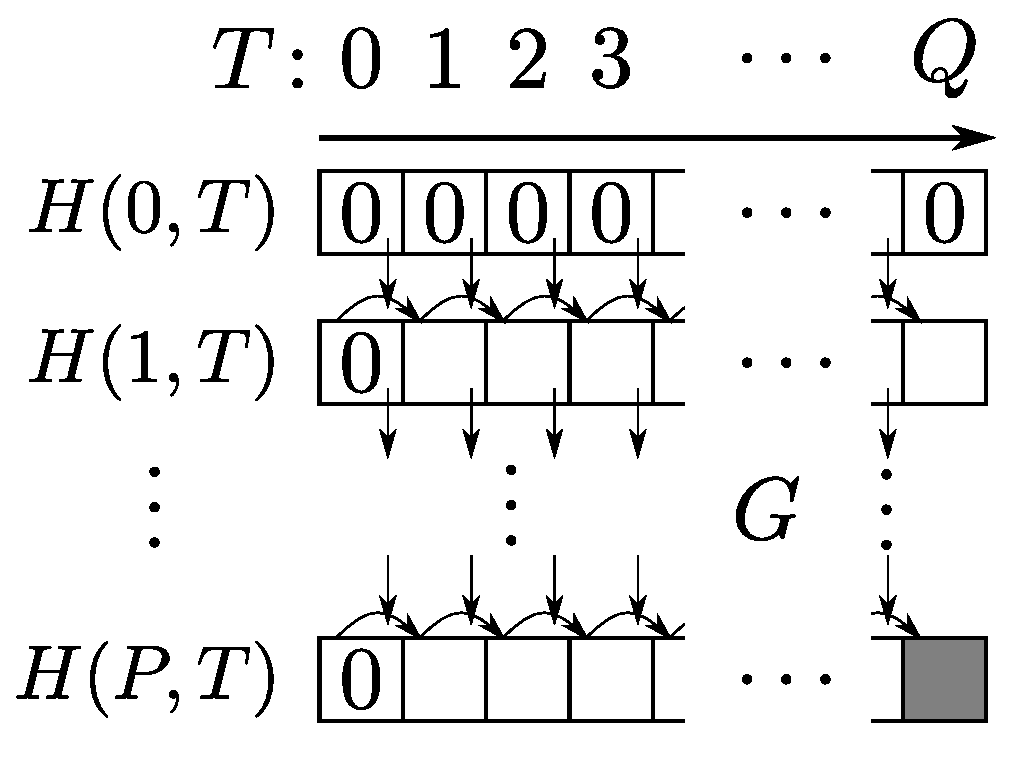
\includegraphics[height=0.2\textheight]{image/divp.eps}
  \end{center}
  \caption{差分方程式と認識される言語}
 \end{figure}

$(G_u)_u$ が{\bf 一様}であるとは,
各 $u$ について $G _u$ の段数, 列数及び欄の大きさが $|u|$ の多項式の指数($2^{\mathrm{poly} (|u|)}$)で抑えられ, 
かつ与えられた $(u, i, T, Y)$ から多項式時間で $G_u(i, T, Y)$ が
計算できることと定義する.
$G_u$ の段数がさらに $|u|$ の多項式で抑えられるとき, 
族 $(G_u) _u$ は\emph{多項式段}であるという. 
河村の論文では次が示されている.

 \begin{lemma}[補題 4.7. \cite{kawamura2010lipschitz}]
  \label{WeakFeedback}
  任意の言語 $L \in \classPSPACE$ に対して,
  その言語を認識する多項式段一様な $(G_u)_u$ が存在する.
 \end{lemma}


\subsection{多項式段一様関数族の差分方程式と$\classPSPACE$}


任意の言語 $L \in \classPSPACE$ について, 
その差分方程式が $L$ を認識する
多項式段一様な関数族 $(G_u)_u$ が存在すること(補題 \ref{WeakFeedback})は
河村によって示されているがその証明の概略を示す.

$\classPSPACE$ 完全な言語である
\textsf{QBF} を認識する $(G_u)_u$ を構成することにより,
任意の $L \in \classPSPACE$ を認識する多項式段一様な関数族 $(G_u)_u$ が存在することを示す.
ここで \textsf{QBF} とは,
文字列 $u$ を $\psi = Q_1 x_1 \cdots Q_n x_n \phi(x_1, \dots, x_n)$ と解釈したとき 
$u \in \textsf{QBF} \Leftrightarrow \psi = T$ によって定義される言語である. 
ただし$Q_i$ は$\exists$ または $\forall$,  
$\phi(x_1, \dots, x_n)$ は $x_i$ 以外の変数を含まない論理式とする. 

論理式 $\psi = Q_1 x_1 \cdots Q_n x_n \phi(x_1, \dots, x_n)$ の値を
$\vee, \wedge$によってラベル付された二分木によって計算することを考える. 
量化子$Q_1 x_1$ を除き $x_1$ を $T$ と $F$ に置き換えた式をそれぞれ
$\psi_T = Q_2 x_2 \cdots Q_n x_n \phi(T, x_2, \dots, x_n)$,
$\psi_F = Q_2 x_2 \cdots Q_n x_n \phi(F, x_2, \dots, x_n)$ と置くと
$Q_1=\forall$ ならば $\psi = \psi_T \wedge \psi_F$, 
$Q_1=\exists$ ならば $\psi = \psi_T \vee \psi_F$.
つまり変数の1つ少ない2つの論理式と量化子によってもとの論理式の値も決まる.
これを再帰的に繰り返すことで $\psi$ は計算可能であり, 
それは深さ $n$ の二分木を葉から根へ値を定めていくことと同じである.
この過程は二分木の深さが段数に, 幅が列数に対応する形で
多項式段一様な関数による差分方程式で模倣可能であるため,
\textsf{QBF} を認識する多項式段一様関数の差分方程式が存在する.


\subsection{多項式段差分方程式を模倣する関数族}


\begin{lemma}
 \label{DifferentiableFamily}
 任意の言語 $L \in \classPSPACE$ に対して, 
 係数のみに $i$ を含む多項式 $\mu_i$ が存在して,
 任意の多項式 $\gamma$ に対して,
 多項式 $\rho$, 関数族 $(g_u)_u, (h_u)_u$ で, 
 $(g_u)_u$ は多項式時間計算可能であり,
 各文字列 $u$ に対して以下を満たすものが存在する.
 \begin{enumerate}
  \item $g_u\colon [0,1] \times [-1,1]\to \R, \quad h_u\colon [0,1] \to [-1,1]$;
  \item $h_u$ は $g_u$ の常微分方程式 (\ref{eq:ode}) の解; 
  \item $g_u$ は $(\infty, 1)$ 階連続微分可能;
  \item 任意の $i \in \N$, $y \in [-1,1]$ に対して
	\begin{equation*}
	 \D{i, 0} g_u(0,y) = \D{i, 0} g_u(1,y) = 0;
	\end{equation*}
  \item \label{enum:infty1}
	任意の $i \in \N$, $j \in \{0,1\}$ に対して
	\begin{equation*}
	 |\D{i,j} g_u| \leq 2^{\mu_i (|u|) - \gamma(|u|)};
	\end{equation*}
  \item $h_u(1) = 2^{-\rho(|u|)}L(u)$.
 \end{enumerate}
\end{lemma}

 この補題より関数族 $(g_u)_u, (h_u)_u$ で $h_u$ は $g_u$ の常微分方程式の解であり,
 $g_u$は滑らかであり, 各 $h_u(1)$ に $L(u)$ の情報を持つものの存在が示される.
 条件 (iii) -- (v) はすべて定理 \ref{DifferentiableIsPspace} の $g$ を
 滑らかな関数とするために必要となる条件である.
 詳細については定理の証明の際に説明する.
 

 この補題の証明の基本的な流れを説明する.
 任意の言語 $L \in \classPSPACE$ に対し, 
 補題 \ref{WeakFeedback} を用いて $L$ を認識する $(G_u)_u$ 
 及びその差分方程式の解 $(H_u)_u$ を得る.
 各 $G_u, H_u$ を模倣する
 滑らかなな $g_u \colon [0,1] \times [-1, 1] \to \R$ 
 とその常微分方程式の解 $h_u \colon [0,1] \to \R$ を構成する.
 また $(G_u)_u$ の一様性から $(g_u)_u$ の多項式時間計算可能性を示す.


 上記の証明は基本的に, リプシッツ連続条件の場合の証明と変わらない.
 違いは $g_u$ を滑らかな関数にするため, 
 以下のような滑らかな多項式時間実関数 $f \colon [0,1] \to \R$ を用いて
 $g_u$ を構成している点である.

 \begin{lemma}[補題 3.6. \cite{ko1991complexity}]
  \label{SmoothFunction}
  以下を満たす多項式時間無限回微分可能実関数 $f \colon [0,1] \to \R$ が存在する.
  \begin{enumerate}
   \item $f(0) = 0, \quad f(1) = 1$;
   \item 任意の $n \ge 1$ で $f^{(n)}(0) = f^{(n)}(1) = 0$;
   \item $f$ は $[0,1]$ で単調増加;
   \item 任意の $n \ge 1$ で $f^{(n)}$ は多項式時間実関数.
  \end{enumerate}
 \end{lemma} 


\subsection{定理 \ref{DifferentiableIsPspace} の証明}

 $\classPSPACE$ 完全な言語 {\sf QBF} 補題 \ref{DifferentiableFamily} から得られる
 $(g_u)_u$ と $(h_u)_u$ から滑らかな $g$ と
 その常微分方程式の解で $\classPSPACE$ 困難な $h$ を構成する.
 各 $h_u(1)$ には $L(u)$ の情報が含まれるため,
 すべての $h_u$ を一つの関数 $h$ に埋め込みたい.
 そこで [0,1] を無限の区間に分割し, $h$ の各文字列 $u$ に対応する区間
 $[l^-_u, c_u]$ に $h_u$ を
 縮小して埋め込む. 
 ただし次の文字列 $u'$ の計算に影響を与えないために,
 $h_u$ を定義域方向について反転したものを
 区間 $[c_u, l^+_u]$ に埋め込むことで影響を相殺する.
 つまり $h(l^-_u) = 0,\ h(c_u) = 2^{-\rho'(|u|)} L(u),\ h(l^+_u) = 0$ を満たす
 ように $h_u(t)$埋め込む.
 ただし $\rho'$ とは $\rho$ に縮小率をかけたものとする.
 同様に $g$ は $h$ が常微分方程式の解となるよう,
 各文字列 $u$ に対応する区間に $g_u$ を縮小して埋め込む.

 リプシッツ連続条件の場合と異なる点は, $g_u$ を構成する時点で
 $(\infty, 1)$ 階連続微分可能にするために,
 $|\D{i,0} g_u|, |\D{i,0} g_u|$ の大きさを制限する点である
 (補題 \ref{DifferentiableFamily} の (\ref{enum:infty1})).
 
